\documentclass{article}
\usepackage[utf8]{inputenc}
\usepackage{fullpage}

\usepackage{hyperref}
\usepackage{subfig}
\usepackage{graphicx}
\usepackage{xcolor}
\let\MYorigsubfloat\subfloat
\renewcommand{\subfloat}[2][\relax]{\MYorigsubfloat[]{#2}}

\newcommand{\sizeBranches}{.49\textwidth}
\newcommand{\figPosition}{h!}

\newcommand{\fourFigBranch}[3]{
    \begin{figure*}[#1]
    \subfloat[]{\includegraphics[width=\sizeBranches]{img/#2_try.pdf}}
    \hfill
    \subfloat[]{\includegraphics[clip, width=\sizeBranches]{img/#2_mozilla_inbound.pdf}}
    \hfill
    \subfloat[]{\includegraphics[clip, width=\sizeBranches]{img/#2_mozilla_central.pdf}}
    \hfill
    \subfloat[]{\includegraphics[clip, width=\sizeBranches]{img/#2_mozilla_release.pdf}}\\
    \caption{\label{#2} #3}
    \end{figure*}
    \newpage
}

\newcommand{\threeTypesBranch}[8]{
\ifx \hideAll \undefined
    \ifx \hideTitle \undefined
        \subsection{All pushes}
    \fi
    #4
    \fourFigBranch{#1}{#2}{#3}
\fi


\ifx \hideMercurial \undefined
    \ifx \hideTitle \undefined
        \subsection{Pushes found on mercurial}
    \fi
    #6
    \fourFigBranch{#1}{#2_MERCURIAL}{#5}
\fi


\ifx \hideCount \undefined
    \ifx \hideTitle \undefined
        \subsection{Pushes NOT found on mercurial}
    \fi
    #8
    \fourFigBranch{#1}{#2_COUNT}{#7}
\fi
}

\def\hideAll{ok}
%\def\hideMercurial{ok}
\def\hideCount{ok}
\def\hideTitle{ok}

\newcounter{QCount}
\newcommand{\kyle}[1]{\textcolor{red}{{\it [Kyle Q\arabic{QCount}\stepcounter{QCount}: #1]}}}

\title{Mozilla's data analysis - intermediate results}
\author{Doriane Olewicki }
\date{May 2019}

\begin{document}

\maketitle


\tableofcontents

\newpage



In this report, we explain in detail the results and graphs that we obtained from the Mozilla build data, as well as potential questions (i.e.: \kyle{a question}). Please, take a look and tell us what you think.

Thanks in advance.

\section{\label{KYLE} Pushes not found in the Mozilla build dataset}

We discovered some interesting facts about the mozilla-central branch. In fact, until now, we always had a figure showing that the mozilla-central branch's number of builds by push varied over time. The median value would vary between 5 and 500 until release 44, then, it would stabilize around 1109, as seen in Fig~\ref{build_push_mozilla_central_alone}.

\begin{figure}[!h]
    \centering
    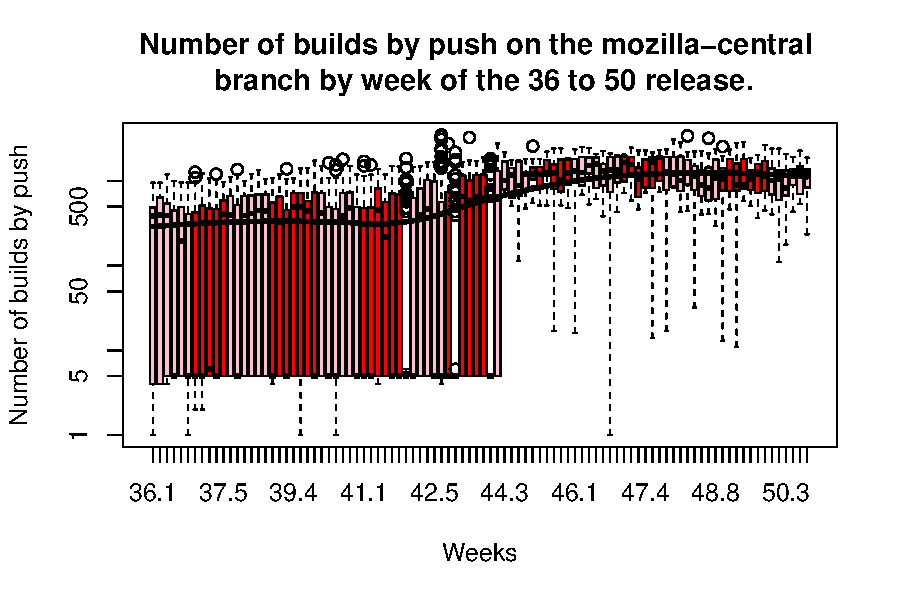
\includegraphics[width=0.45\textwidth]{img/build_push_mozilla_central.pdf}
    \caption{The number of builds by push on the mozilla-release branch varies overtime. Two states, the first one having the median varying between 5 and 500, the second one, after release 44, being around 1109.}
    \label{build_push_mozilla_central_alone}
\end{figure}

However, when we mined the mercurial mozilla-central repository and counted the number of commits for each push when associating the pushes found for the Fig~\ref{build_push_mozilla_central_alone} to those in the mercurial repository, only 57\% (1987 out of 4697) of the pushes were retrieved. That number seems odd, since, on the other branches, about 98\% of the pushes were retrieved, using the same technic.

\begin{figure}[!h]
    \centering
    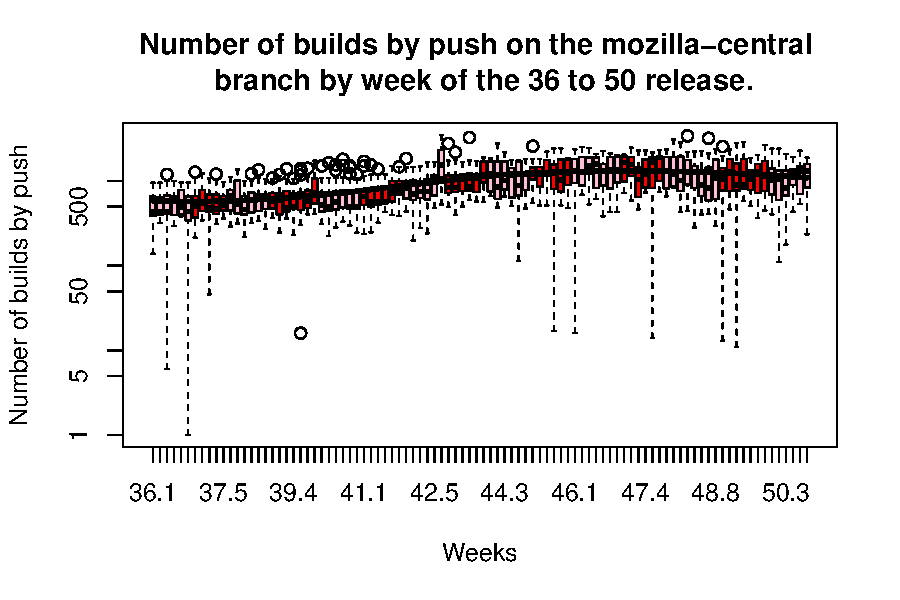
\includegraphics[width=0.45\textwidth]{img/build_push_MERCURIAL_mozilla_central.pdf}
    \caption{The number of builds by push on the mozilla-release only for the pushes \textbf{present on the mercurial repository.}}
    \label{build_push_MERCURIAL_mozilla_central_alone}
\end{figure}

To analyze this, we decided to generate the same figure as Fig~\ref{build_push_mozilla_central_alone} but only showing the pushes that were found on the mercurial repository. On the Fig~\ref{build_push_MERCURIAL_mozilla_central_alone}, we can thus see the results of that selection. The curve is here much smoother and all the pushes having 5 builds seem to have been removed.

\begin{figure}[!h]
    \centering
    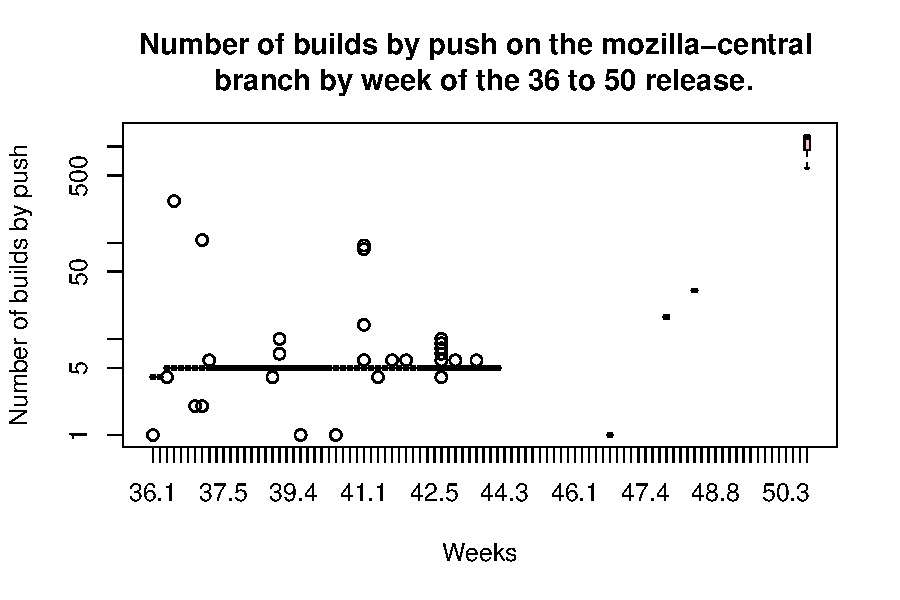
\includegraphics[width=0.45\textwidth]{img/build_push_COUNT_mozilla_central.pdf}
    \caption{The number of builds by push on the mozilla-release only for the pushes \textbf{NOT present on the mercurial repository.}}
    \label{build_push_COUNT_mozilla_central_alone}
\end{figure}

If we invert the selection, selecting only the number of builds of the pushes not found on the repository, it confirms that most of the pushes that were removed are pushes that have 5 builds (cf. Fig~\ref{build_push_COUNT_mozilla_central_alone}).

In fact, there are 1886 pushes that all run the same 5 builds : 

\begin{itemize}
    \item Firefox mozilla-central linux l10n dep  
    \item Firefox mozilla-central linux64 l10n dep 
    \item Firefox mozilla-central macosx64 l10n dep    
    \item Firefox mozilla-central win32 l10n dep    
    \item Firefox mozilla-central win64 l10n dep 
\end{itemize}


\kyle{What are those pushes that are not retrieved from the mercurial repositories ?} 

\kyle{What are the "l10n dep" builds?}

In the rest of the report, only the data regarding the pushes we found on mercurial is used. See the first part of this report for more explanations.

\newpage
%\section{Introduction}

%In this report, we gathered the results we generated the last few weeks. 

%First, for the first four sections, we showed 3 groups of graph each time, let me explain here where this separation comes from. Each push is identified by a \texttt{revision\_12C}, which is the revision number of the last commit in that push. To count the number of commits by push, we gathered commits from mercurial regarding the studied period. Most of the \texttt{revision\_12C} from the initial dataset (retrieved by Nourredine) was found in the data scrapted from mercurial : 98\% of the \texttt{revision\_12C} are retrieved, covering 99.8\% of the builds. 

%Hovewer, the numbers are much different when looking at the "mozilla-central" branch, where only 57\% of the \texttt{revision\_12C} are retrieved, still covering 99.4\% of the builds. The remaining 43\% have only a low number of builds and are mainly in releases 36 to 44. See Fig~\ref{build_push_COUNT}(c) to visualise that.

%Also, it must be known that an initial count of commit by push had been done by Nourredine in the first dataset, under the name \texttt{count\_elements}. This values often differ from the mercurial dataset, differ from one build to an other even if the commit didn't changed and does sometimes omit some commits or add others. I still need to check on that.

%Thus, I computed the number of commits by push using 3 differents ways :
%\begin{itemize}
%    \item using the count from the mercurial scrap and using the \texttt{count\_elements} highest value for each \texttt{revision\_12C};
%    \item using the count from the mercurial scrap and ignoring the \texttt{revision\_12C} unfound on mercurial;
%    \item using the \texttt{count\_elements} highest value for each \texttt{revision\_12C}.
%\end{itemize}

%That's why each group of graph is represented three times. 


\newpage
\section{Overview of the build data}

\begin{figure*}[!h]
\subfloat[]{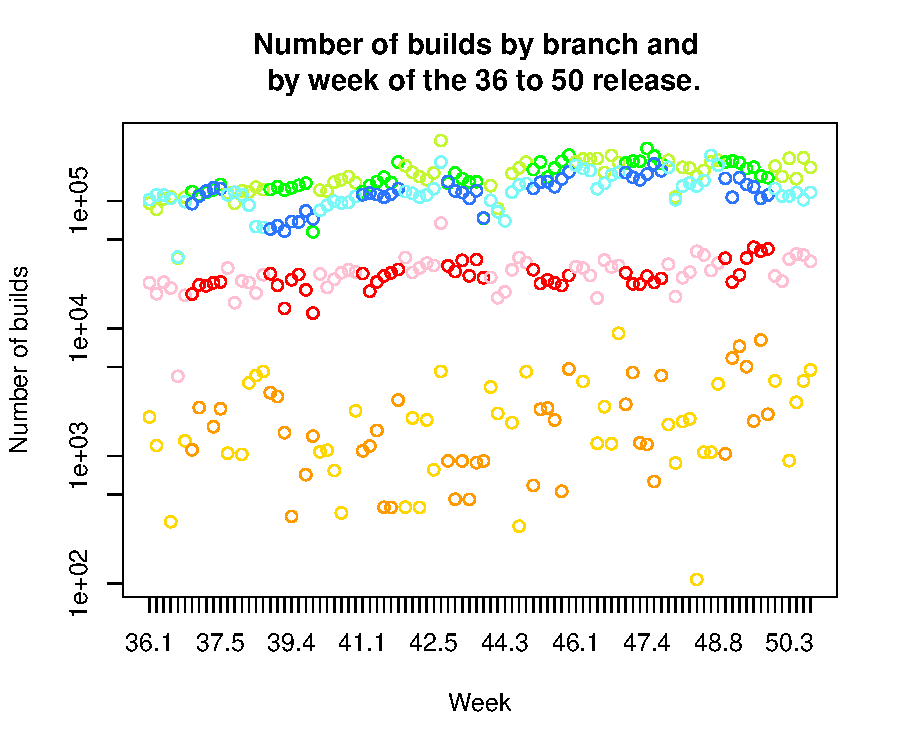
\includegraphics[clip, width=0.3\textwidth]{img/build_week.pdf}}
\hfill
\subfloat[]{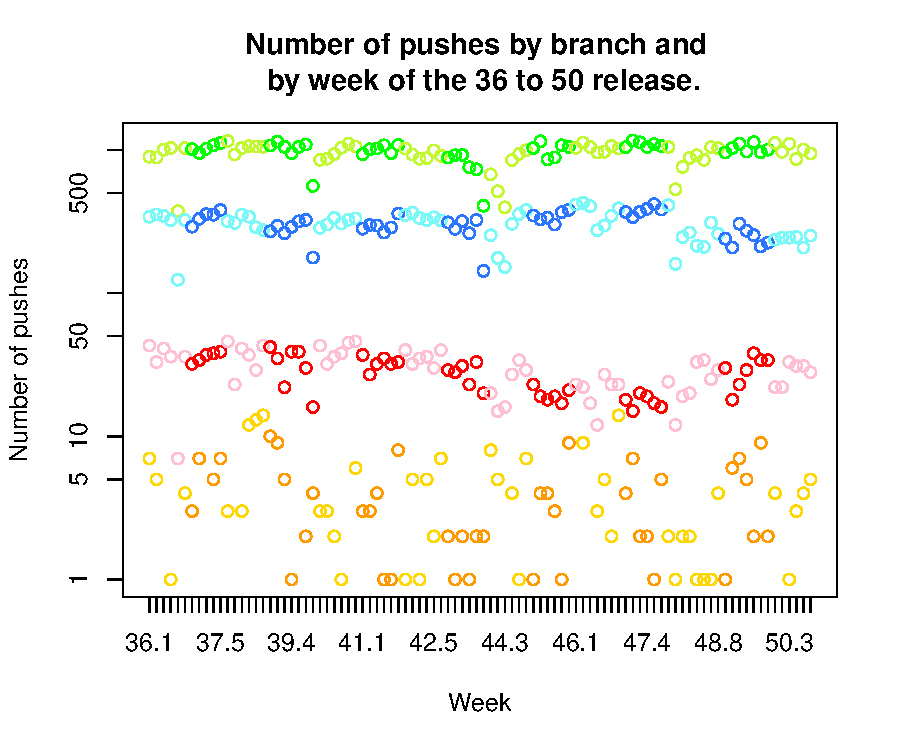
\includegraphics[clip, width=0.3\textwidth]{img/push_week.pdf}}
\hfill
\subfloat[]{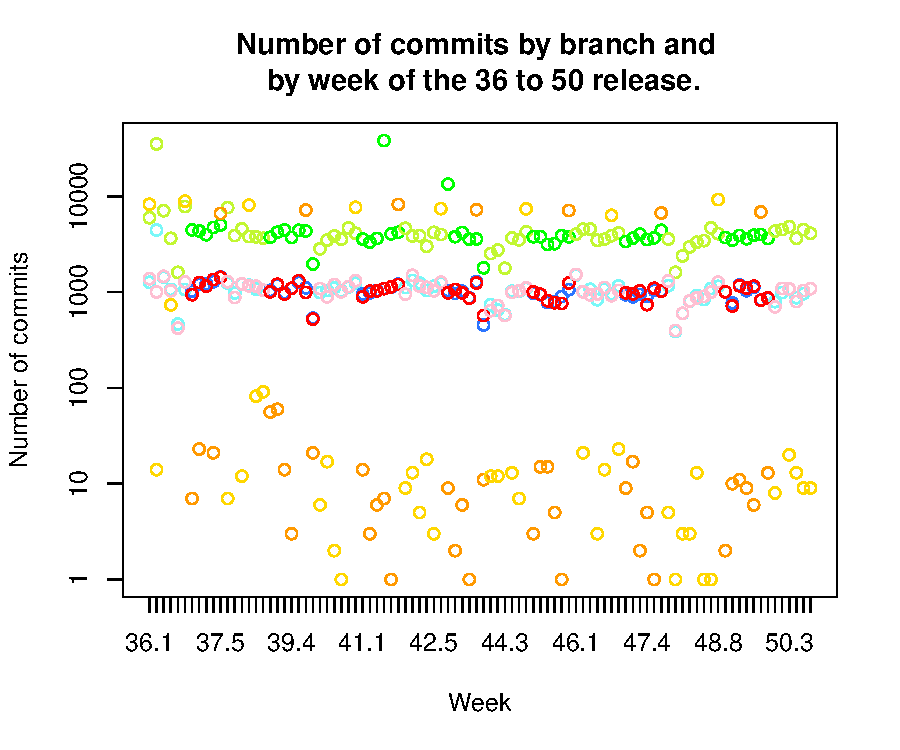
\includegraphics[clip, width=0.3\textwidth]{img/commit_week.pdf}}\\
\caption{\label{byweek}Quantitative values by week computed on the build dataset. (a) Number of builds by week. (b) Number of pushes by week. (c) Number of commits by week. }
\end{figure*}



%\kyle{The higher number of pushes from release 36 to 44 on the mozilla-central branch on Fig~\ref{byweek}(a) would reduce and be more stable over time if we would ignore the pushes not found on mercurial (43\% of the pushes of that branch, see the first two pages of the report). For the rest, does those results seems logical to you regarding the purpose of each branch ?}

\kyle{Do those results seem logical to you regarding the purpose of each branch ? }
\newpage
\section{BUILD x PUSH}
\label{build_push_sec}

For this first section we just gathered the number of builds by push, identified by a different \texttt{revision\_12C} by push. 

\threeTypesBranch{h}{build_push}
{
    Number of builds by commit on each branch. (a) The median is at 52 builds and is quite stable across time. (b) The median is at 305 builds and is quite stable across time.  (c) The median has two stable states and goes from the first one to the other at release 44. The median is at 5, then goes up to 1109 from release 44. (d) The median grows exponentially, starting at 306 during release 36 and going up to 920 during release 50.
}
{
    Looking at all the pushes, disregarding if we found it on the mercurial or not, we can see that the "try" and "mozilla-inbound" branches are quite stable, having a slight increase over time. On the "mozilla-central" branch, the behaviour changes over time, the mean increasing a lot. The "mozilla-release" branch shows an exponential increase overtime.
}
{  
    Number of builds by commit on a log scale on each branch for pushes that were found on mercurial. (a) The median is at 52 builds and is quite stable across time. (b) The median is at 305 builds and is quite stable across time.  (c) The median has two stable states and goes from the first one to the other at release 44. The median is at 669, then goes up to 1234 from release 44. (d) The median grows exponentially, starting at 306 during release 36 and going up to 920 during release 50.
}
{
    %Same behaviour as before for the "try", "mozilla-inbound" and "mozilla-release" branches. The "mozilla-central" branch's behaviour changes a lot regarding the privious graph.
    We can see that the "try" and "mozilla-inbound" branches are quite stable, having a slight increase over time. On the "mozilla-central" branch, the behaviour changes over time, the median increasing a lot. The "mozilla-release" branch shows an exponential increase overtime.
    
    \kyle{We believe the increase over time is due to more and more tests being added to the builds sets. Is that the right explanation for you too ?} 
    
    \kyle{What happened around release 44 on the mozilla-central branch ? The number of builds by push increasing slows down.}
}
{
    Number of builds by commit on each branch for pushes that were not found on mercurial. (a) The median is at 1 build with some peaks overtime. Some weeks have no push missing on mercurial. (b) The median is at 1 build with some peaks overtime. Some weeks have no push missing on mercurial. (c) The median has two stable states and goes from the first one to the other at release 44. The median is at 5, then, no pushes are missed on mercurial from release 44. Some out-layers appear overtime. (d) All pushes were found on this branch but for the last release, having a peak at 923 builds.
}
{
    This shows that among the pushes not found on mercurial, most of them have a really low number of builds. This shows also that the large variations in Fig~\ref{build_push}(c) over releases 36 to 43 come from the the unfounded pushes.
}

\section{COMMIT x PUSH}
\label{commit_push_sec}
\threeTypesBranch{h}{commit_push}
{
    Number of commits by push on each branch. (a) The median is at 1 commit. (b) The median is at 1 commit. (c) The median has two stable states and goes from the first one to the other at release 44. The median is at 18, then goes up to 22 from release 44 and varies a lot more. (d) The median is at 2 across time but as peaks at ends of releases.
}
{
    For each push in the build data, we computed the number of commits in the push by counting the changesets in mercurial for the corresponding push. If the push is not retrieved in the mercurial dataset, we took the number of changesets already given by the build dataset.
}
{
    Number of commits by push on a log scale on each branch for pushes that were found on mercurial. (a) The median is at 1 commit. (b) The median is at 1 commit. (c) The median is at 23. The number of commits varies a lot more. (d) The median is at 2 across time but as peaks at ends of releases that goes up to 10~000 commits.
}
{
   For each push in the build data, we computed the number of commits in the push by counting the changesets in mercurial for the corresponding push. We only displayed the counts for the pushes retrieved in the mercurial dataset (see Section~\ref{KYLE}).
   
   The median number of commits by push is at 1 for the try and mozilla-inbound branch. The median is higher for the mozilla-central branch where commits are gathered. Then, the mozilla-release branch shows peaks or large outliers around the end of releases.
   
   \kyle{Median at 1 for the try branch and the mozilla-inbound branch, does it seem right ?}
}
{
    Number of commits by push on each branch for pushes that were not found on mercurial. (a) The median is at 19 commits. (b) The median is at 8 commits. (c) The median is at 10 commits. (d) The median is at 8 commits.
}
{
    In this last subsection, we showed the number of commits by push for all the pushes in the build data if we took the count given by that dataset. The results have different behaviors.
}

\section{BUILD x COMMIT}

To compute the number of builds by commit, we took the number of builds by push computed in section~\ref{build_push_sec} and the number of commits by push computed in section~\ref{commit_push_sec}. By dividing the number of builds with the number of commits for each push, we could have the new results.


\threeTypesBranch{h}{build_commit}
{
    Number of builds by commit on each branch. (a) The median is at 23 builds and is quite stable across time. (b) The median is at 213 builds and is quite stable across time.  (c) The median has two stable states and goes from the first one to the other at release 44. The median is at 0.5, then goes up to 34 from release 44. (d) The median grows exponentially, starting at 102 during release 36 and going up to 725 during release 50.
}
{
    In this section we show the results for all the pushes, disregarding the availability of the push in the mercurial dataset. 
}
{
    Number of builds by commit on a log scale on each branch for pushes that were found on mercurial. (a) The median is at 23 builds and is quite stable across time. (b) The median is at 214 builds and is quite stable across time.  (c) The median is at 33. (d) The median grows exponentially, starting at 102 during release 36 and going up to 917 during release 50.
}
{
    We only show the results for the pushes that were retrieved in the mercurial dataset.
    
    Try and mozilla-central branches have a quite low median number of builds by commit, respectively 23 and 33. The mozilla-inbound has a quite high median number, at 214. Finally, the mozilla-release has a really high median number, with peaks and ouliers much lower at ends of releases. This is due to the upward peaks in section~\ref{commit_push_sec}.
    
    \kyle{Why mozilla-central as such a low number of builds by commit, compated to mozilla-inbound and mozilla-release ?}
}
{
    Number of builds by commit on each branch for pushes that were not found on mercurial. (a) The median is at 3 builds and is quite stable across time. (b) The median is at 27 builds and is quite stable across time.  (c) The median has two stable states and goes from the first one to the other at release 44. The median is at 0.5, then goes up to 81 from release 44. (d) The median grows exponentially, starting at 36 during release 36 and going up to 114 during release 50.
}
{
    The results here are computed by taking the number of commits by push given by the build dataset.
}
\section{PRICE x COMMIT}

\subsection{Hypothesis for the cost computation}

In this analysis, we wanted to estimate the cost of a commit regarding the builds generated. To do so, we made some assumptions that are explained in this section.

The Linux platform builds are run on Amazon AWS, for which the tarification is available. The other platforms, Windows and MacOS, are run in house, so the cost is computed differently, see below.

To compute the cost of each commit, the formula used is the following :

$$\frac{\sum_{p\in Platforms} (C_{1p}\sum_{c \in build_{cp}} T_{c} + C_{2p}\sum_{t \in build_{tp}} T_{t})}{\#commit\_in\_push}$$

Where $C_{1j}$ is the cost of the compilation builds for the $j$ platform associated with the commit, $C_{2j}$ is the cost of the testing builds for the $j$ platform associated with the commit, $build_{i j}$ are all the builds of the build $i$ type for the $j$ platform associated to the commit and $T_i$ in the time of the build $i$.

\subsection{Linux platform cost}

The cost of the Linux platform comes from the Amazon AWS tarification. We selected the On Demand prices which is estimated at USD~0.45 per hour for compilation builds and USD~0.12 per hour for testing builds. This numbers come from a blog article from 2013 that used those to estimate the same costs.

\subsection{MacOS and Windows platforms cost}

Regarding the MacOS and Windows platforms, we want to evaluate the cost by evaluating the cost of having physical machines, maintaining them and the energy consumed. We want to estimate that cost using data we have from the IT department at Polytechnique Montréal as well as data available online. 

\kyle{However, if you have any of that information about Mozilla, it would be really helpful for more accurate cost evaluations.} 

The cost of those platforms is composed of three cost : the machine cost, the energy cost and the developer's salary cost. 

The machine cost is estimated at CAD 1530 without taxes, cost of the machines at Polytechnique Montréal. Knowing that the taxes in Canada are around 15\% and the exchange rate is 0.76, the cost of a machine is $1530 \cdot 1.15 \cdot 0.76=1337.22$ USD. The machines are estimated to be changed every five years. To compute the by hour cost,  we have to divide the cost by five for the five years of use, by 365 for the days by year and by 24 for the hours of the day. 

$$\textit{Machine cost = } 1337.22~[USD] / 5 / 365 / 24 = 0.0305~[USD]$$

Regarding the energy cost, using Polytechnique Montréal's data, the machines consume 1kWh in 4 hours. From online data \footnote{\url{https://www.chooseenergy.com/electricity-rates-by-state/}, consulted the 07/11/2019.}, the mid cost of energy in the US is 13.26cents by kWh.

$$\textit{Energy cost = } 1~[kWh] / 4 \cdot 0.1326~[USD/kWh] = 0.03315~[USD]$$

The mid developer's salary in the US is 118k USD \footnote{\href{https://www.lemagit.fr/actualites/450412783/Selon-Hired-les-salaires-des-developpeurs-en-Europe-restent-tres-inferieurs-aux-salaires-US}{https://www.lemagit.fr/actualites/450412783/Selon-Hired-les-salaires-des-developpeurs-en-Europe-restent-tres-inferieurs-aux-salaires-US}, consulted the 07/15/2019.}. We estimate that a developer is responsible of 100 machines. The computation of the salary by hour is computed by dividing by 365 (number of days by year) and by 24 (number of hours by day).

$$ \textit{Salary cost = }118k~[USD] / 100 / 365 / 24 = 0.1347~[USD] $$ 

The total cost by hour is thus estimated at USD~0.198.

\subsection{Results}

%\threeTypesBranch{h}{price_commit}
%{
%    Price by commit on each branch. (a) The median is at 24~USD and is quite stable across time. (b) The median is at 212~USD and is quite stable across time.  (c) The median has two stable states and goes from the first one to the other at release 44. The median is at 0.8~USD, then goes up to 35~USD from release 44. (d) The median grows exponentially, starting at 104~USD during release 36 and going up to 693~USD during release 50.
%}
%{
%    
%}
%{
%    Price by commit on each branch for pushes that were found on mercurial. (a) The median is at 1.5~USD and is quite stable across time. (b) The median is at 15~USD and is slightly increasing across time.  (c) The median is at 2~USD. (d) The median grows exponentially, starting at 12~USD during release 36 and going up to 60~USD during release 50.
%}
%{
%    \kyle{Here we can see results with more flexible assumption, supposing that all builds' platforms would have costs similar to the AWS tarification. What do you think about that ?}
%    
%    The cost increases slightly on all the branches, most visibly is on the mozilla-release branch. Each commit costs about 2~USD on the try and mozilla-central branches. The mozilla-inbound branch has 15~USD commits and the mozilla-release branch has even more expensive commits.
%}
%{
%    Price by commit on each branch for pushes that were not found on mercurial. (a) The median is at 24~USD and is quite stable across time. (b) The median is at 212~USD and is quite stable across time.  (c) The median has two stable states and goes from the first one to the other at release 44. The median is at 0.8~USD, then goes up to 35~USD from release 44. (d) The median grows exponentially, starting at 104~USD during release 36 and going up to 693~USD during release 50.
%}
%{
%    
%}

\fourFigBranch{h}{price_commit_MERCURIAL}{
Price by commit on each branch for pushes that were found on mercurial. (a) The median grows overtime, starting at 1.4~USD during release 36 and going up to 2~USD during release 50. (b) The median is at 17~USD and is slightly increasing across time.  (c) The median grows exponentially, starting at 1.5~USD during release 36 and going up to 3.5~USD during release 50. (d) The median grows exponentially, starting at 25~USD during release 36 and going up to 56~USD during release 50.
%[1] "try"              "1.90926142759117"
%[1] "mozilla-inbound"  "16.8500618841536"
%[1] "mozilla-central"  "2.49681245034413"
%[1] "mozilla-release"  "27.9942335697263"
}


\textcolor{white}{empty}
\newpage
\section{WAIT x PUSH}

Waiting time between the push and the build is computed by taking the difference between last commit in the push's time and the first build starttime. The first commit in the build's time is not in the data I retrieved from mercurial since only the last commit time is given. 

To be able to show a significant plot, we wanted to have a logarithmic scale. We thus had to add 1min to every delay to be able to do so. The median were computed without that additional minute.

We can see that on each branch, two tendencies alternate : the first one at 1min, the second one at 61min. I wonder if their might be a difference on the time encoding during the 61min tendency, regarding the timezone. First transition was end 22nd of June 2015 (r39.6 to r39.7), second was 26th of October 2015 (r42.5 to r42.6), the third was 20nd of June 2016 (r48.2 to r48.3) and the last the 24th of October 206 (r50.5 to r50.6).

\kyle{Do you know if there might be a difference in the timezone that brought that difference in the tendencies ? Or do you think there is an other reason for that alternation ?}

There is still a lot of out-layers higher than the median.





\fourFigBranch{h}{wait_push}{}
\section{TYPE x RESULT}

Globally, a huge number of tests succeed. The number of successful test seems to increase overtime on all branches, where the number of compilation and test fails stays quite stable. The numbers fluctuate a lot from one week to another.

\fourFigBranch{h}{type_result}{Number of builds by type and results on each branch.}

\section{TYPE x PLATFORM}

Globally more tests than compilations.

\fourFigBranch{h}{type_platform}{Number of builds by type of builds and platform by week. (a) Most tests on the linux platform, then Windows, then MacOS. The number of tests also increases overtime on all platforms. The number of compilation are quite similar on each platform, linux being a little higher. (b) Similar number of tests on the Linux and Windows platforms, lower on the MacOS platform.}
\section{PLATFORM x RESULT}

Globally more success than failure.

\fourFigBranch{h}{platform_result}{Number of builds by platform and result on each branch. (a) Linux, Windows then MacOS. (b) Linux and Windows are similar, MacOS is lower. (c) Linux and Windows are similar, MacOS is lower. (d) Differences between platforms are less visible.}
\section{PLATFORM FAILS}

This section is similar to the previous section, but it only shows failed builds.  

\fourFigBranch{h}{platform_fail}{Number of failed builds by platform. (a) Linux is the highest, then Windows, then MacOS. (b) Linux is similar to Windows , except from r41 to r44 where Linux was higher. (c) Mac globally lower. Linux and Windows similar, except for some peaks. (d) Low number of failure, multiple peaks on each platform.}
\section{REASON for build triggering}

Mostly scheduled builds, some other types. On the try branch, many "Self-serve" builds, since some builds are asked for by developers on that branch.

\kyle{Do you know what the builds reason mean? We understand the "scheduler" which are scheduled builds and "self-serve" which are builds manually asked for by developers. But we do not understand the others.}

\fourFigBranch{h}{reason}{Number of builds by reason for the build generation.}
\section{Number of pushes/builds BY HOUR OF THE DAY}

More pushes and builds during the night for the try and mozilla-inbound branches then during the day. 

Regarding the mozilla-central and mozilla-release branches, the number of pushes is stable over the hours of the day, but for midnight where there is a down-peak. The number of builds goes down during the morning and there is a peak in both branches at 1 pm.

\kyle{Could you explain these behaviors?}

\begin{figure*}[h]
    \subfloat[]{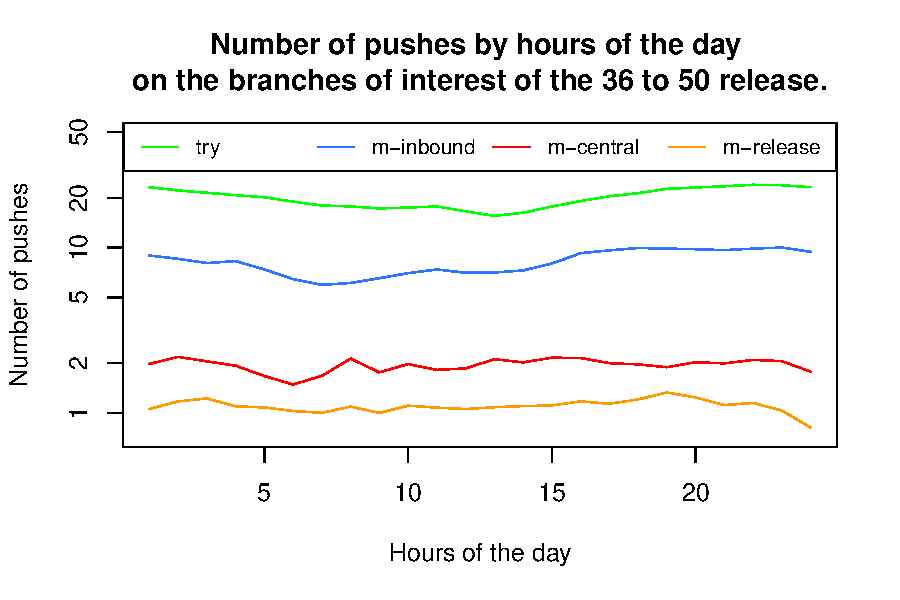
\includegraphics[width=\sizeBranches]{img/push_hour.pdf}}
    \hfill
    \subfloat[]{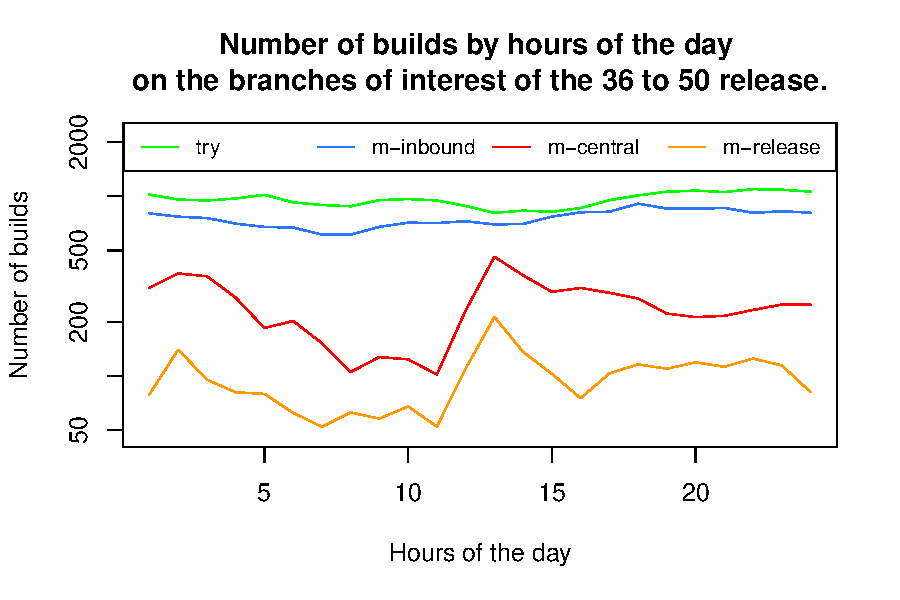
\includegraphics[clip, width=\sizeBranches]{img/build_hour.pdf}}\\
    \caption{\label{hour} Number of (1) pushes and (2) builds by hour of the day on each of the branches of interest.}
\end{figure*}


\section{Number of pushes/builds BY DAY OF THE WEEK}

For all the branches, the numbers go down during the night, stable during the day. 

\kyle{Last Skype meeting, you explained the stability during the day by the resource limitation. No more resource is available, that is why the numbers do not increase further up. Can you confirm?}
\begin{figure*}[h]
    \subfloat[]{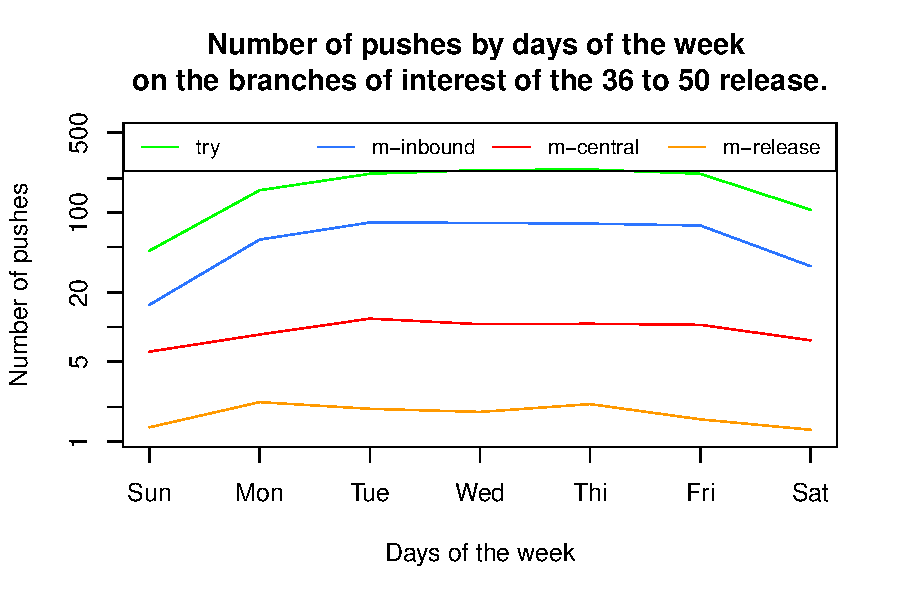
\includegraphics[width=\sizeBranches]{img/push_dayweek.pdf}}
    \hfill
    \subfloat[]{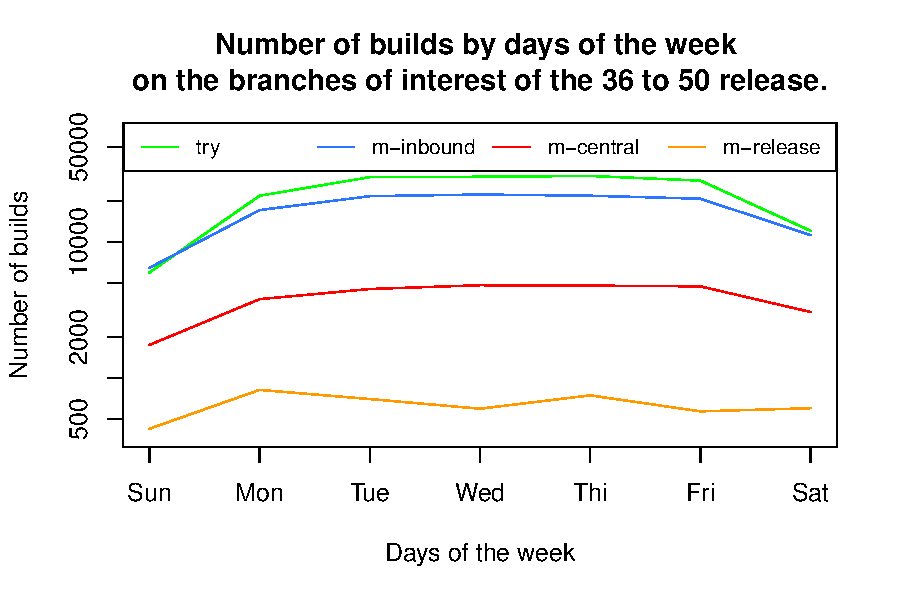
\includegraphics[clip, width=\sizeBranches]{img/build_dayweek.pdf}}\\
    \caption{\label{hour} Number of (1) pushes and (2) builds by day of the week on each of the branches of interest.}
\end{figure*}

\newpage
\section{Analysis of the scheduled compilations}

In this section, we looked closer to compilation builds that were scheduled. The point of that is to identified the scheduler pattern regarding those builds. In the first subsection, all compilation builds are considered as similar. In the second one and third one, the builds are separated, regarding their specificities (type of compilation, platform...).




\subsection{NUMBER OF BUILDS BY WEEK, disregarding the specificities of the builds}


\kyle{Why does it decrease like that ? Why is there such a difference from one week to another?}

\fourFigBranch{h}{build_rw}{Number of scheduled builds (compilations) by week. Global reduction of the number of compilation by week on all branches.
(a) Drops from 6600 at r36 to 3800 during r50.
(b) Stable at 3000 until r46 where it decreases linearly until reaching 2100 during r50.
(c) Drops from 400 at r36 to 260 during r50.
(d) Between 0  and 50 overtime.}






\subsection{NUMBER OF BUILDS BY WEEK, separating builds by specificities}

\kyle{Here, we separated each buildername and printed a line for each of them. Some do stop earlier (i.e. there are more lines on Fig~\ref{build_rw_SEP}(a) before r44). How come ? On the Fig~\ref{cumul_build_rw_SEP}, it will be even more visible. And why are there down- and up-peaks ?}

\kyle{why no pgo on the mozilla-release branch ?}

\fourFigBranch{h}{build_rw_SEP}{Number of scheduled builds (compilations) by buildername by week. 
}





\subsection{CUMULATIVE NUMBER OF BUILDS BY WEEK, separating builds by specificities}

\kyle{Here, we separated each buildername again, but applied a cumulative sum on the number of builds by week, so that the time at which buildernames are stopping or starting appear more clearly. Fig~\ref{cumul_build_rw_SEP}(a) shows multiple builds stopping before release 44 and Fig~\ref{cumul_build_rw_SEP}(d) shows builds starting after release 48. Why?}

\fourFigBranch{h}{cumul_build_rw_SEP}{Cumulative number of scheduled builds (compilations) by buildername by week. 
}





% \section{SHEDULED COMPILATION BUILDERNAME}

\subsection{CUMULATIVE BUILD, Together, all compilation}
\fourFigBranch{h}{cumulative_build_TOG}{Cumulative number of scheduled builds by buildername by time. 
(a) 
(b) 
(c) 
(d)}


\subsection{CUMULATIVE BUILD, Separated, all compilation}
\fourFigBranch{h}{cumulative_build_SEP}{Cumulative number of scheduled builds by buildername by time. 
(a) 
(b) 
(c) 
(d)}


\subsection{CUMULATIVE BUILD, Together (approximated 10\%), all compilation}
\fourFigBranch{h}{cumulative_build_TOG_10}{Cumulative number of scheduled builds by buildername by time. 
(a) 
(b) 
(c) 
(d)}


\subsection{CUMULATIVE BUILD, Separated (approximated 10\%), all compilation}
\fourFigBranch{h}{cumulative_build_SEP_10}{Cumulative number of scheduled builds by buildername by time. 
(a) 
(b) 
(c) 
(d)}

\subsection{BUILD X DAYS, Together (approximated 10\%), all compilation}
\fourFigBranch{h}{build_minutes_TOG_10}{Number of scheduled builds by day and by buildername by time.
(a) 
(b) 
(c) 
(d)}


\subsection{BUILD X DAYS, Separated (approximated 10\%), all compilation}
\fourFigBranch{h}{build_minutes_SEP_10}{Number of scheduled builds by day and by buildername by time. 
(a) 
(b) 
(c) 
(d)}
% \section{Interesting : with points on the boxplot}

\subsection{BUILD x PUSH}
\fourFigBranch{h}{build_push_POINT}{todo}

\subsection{COMMIT x PUSH}
\fourFigBranch{h}{commit_push_POINT_COUNT}{todo}

\subsection{BUILD x COMMIT}
\fourFigBranch{h}{build_commit_POINT_COUNT}{todo}
\end{document}
